\documentclass[tikz,border=2pt]{standalone}
\usepackage[T1]{fontenc}
\usepackage[scaled=0.92]{helvet}
\renewcommand{\familydefault}{\sfdefault}
\usepackage{amsmath,amssymb}
\renewcommand{\tiny}{\fontsize{6.5}{7.5}\selectfont}
\renewcommand{\scriptsize}{\fontsize{7.5}{8.5}\selectfont}
\usetikzlibrary{arrows.meta,fit,backgrounds,calc}
\definecolor{cOK}{HTML}{009E73}
\definecolor{cNo}{HTML}{C0392B}
\definecolor{cInk}{HTML}{22303C}
\definecolor{cGrp}{HTML}{0072B2}
\definecolor{cCl}{HTML}{CFE0F1}
\tikzset{
  every node/.style={font=\scriptsize, text=cInk},
  ev/.style={draw=cInk!70, rounded corners=2pt, minimum height=0.5cm, minimum width=0.85cm, inner sep=1pt},
  live/.style={ev, fill=cOK!16},
  dead/.style={ev, fill=cNo!14, draw=cNo!80, dashed,
     path picture={\draw[cNo!85, thick] (path picture bounding box.south west)--(path picture bounding box.north east);
                   \draw[cNo!85, thick] (path picture bounding box.north west)--(path picture bounding box.south east);}},
  cver/.style={ev, fill=cCl, minimum width=1.05cm},
  cstale/.style={ev, fill=cNo!14, draw=cNo!80, minimum width=1.05cm},
  aok/.style={ev, fill=cOK!16, minimum width=1.05cm},
  ablk/.style={ev, fill=cNo!14, draw=cNo!80, minimum width=1.05cm},
  arr/.style={-{Stealth[length=3.5pt,width=2.6pt]}, thick, draw=cInk!75},
  darr/.style={-{Stealth[length=3.5pt,width=2.6pt]}, thick, draw=cInk!75, dashed},
  rarr/.style={-{Stealth[length=3.5pt,width=2.6pt]}, very thick, draw=cInk!85},
}
% #1..#5: styles of E1 E2 E3 P Q ; #6 claim style; #7 assertion style; #8 title; #9 result text
\newcommand{\panel}[9]{%
\begin{scope}
\path[draw=cGrp, dashed, rounded corners=3pt, fill=cGrp!7] (-0.62,0.28) rectangle (0.62,1.72);
\path[draw=cGrp, dashed, rounded corners=3pt, fill=cGrp!7] (-0.62,-0.72) rectangle (0.62,-0.1);
\node[font=\tiny\bfseries, text=cGrp, anchor=north east, inner sep=0.5pt] at (0.6,1.7) {$S_1$};
\node[font=\tiny\bfseries, text=cGrp, anchor=north east, inner sep=0.5pt] at (0.6,-0.1) {$S_2$};
\node[#1] (e1) at (0,1.32) {$E_1$};
\node[#2] (e2) at (0,0.68) {$E_2$};
\node[#3] (e3) at (0,-0.4) {$E_3$};
\node[#4] (p) at (1.75,1.55) {$P$};
\node[#5] (q) at (1.75,-0.55) {$Q$};
\node[#6] (c) at (1.95,0.5) {$C$};
\node[#7] (a) at (3.1,0.5) {$A$};
\draw[arr] (0.62,1.0) -- (c.north west);
\draw[arr] (0.62,-0.4) -- (c.south west);
\draw[rarr] (p.south) -- (p.south |- c.north);
\draw[darr] (q.north) -- (q.north |- c.south);
\draw[darr] (c.east) -- (a.west);
\node[font=\scriptsize\bfseries, anchor=south] at (1.5,1.95) {#8};
\node[font=\tiny, anchor=north, align=center, text width=3.6cm] at (1.5,-1.0) {#9};
\end{scope}}
\begin{document}
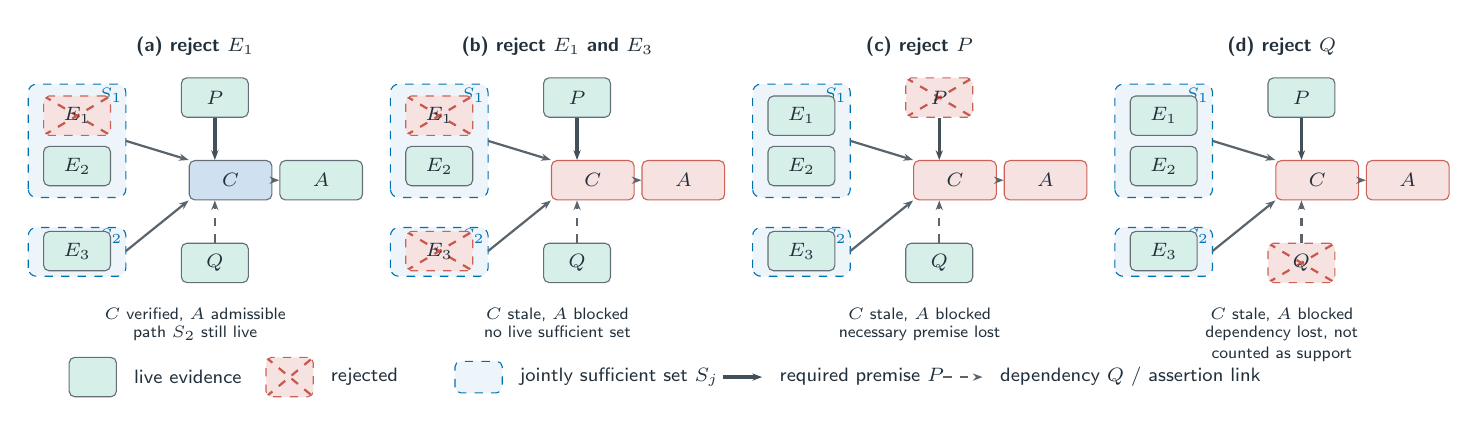
\begin{tikzpicture}
\begin{scope}[shift={(0,0)}]\panel{dead}{live}{live}{live}{live}{cver}{aok}{(a) reject $E_1$}{$C$ verified, $A$ admissible\\[-1pt]{\tiny path $S_2$ still live}}\end{scope}
\begin{scope}[shift={(4.6,0)}]\panel{dead}{live}{dead}{live}{live}{cstale}{ablk}{(b) reject $E_1$ and $E_3$}{$C$ stale, $A$ blocked\\[-1pt]{\tiny no live sufficient set}}\end{scope}
\begin{scope}[shift={(9.2,0)}]\panel{live}{live}{live}{dead}{live}{cstale}{ablk}{(c) reject $P$}{$C$ stale, $A$ blocked\\[-1pt]{\tiny necessary premise lost}}\end{scope}
\begin{scope}[shift={(13.8,0)}]\panel{live}{live}{live}{live}{dead}{cstale}{ablk}{(d) reject $Q$}{$C$ stale, $A$ blocked\\[-1pt]{\tiny dependency lost, not counted as support}}\end{scope}
% legend
\begin{scope}[shift={(0.2,-2.0)}]
\node[live, minimum width=0.6cm] at (0,0) {}; \node[anchor=west] at (0.4,0) {live evidence};
\node[dead, minimum width=0.6cm] at (2.5,0) {}; \node[anchor=west] at (2.9,0) {rejected};
\path[draw=cGrp, dashed, rounded corners=2pt, fill=cGrp!7] (4.6,-0.2) rectangle (5.2,0.2); \node[anchor=west] at (5.3,0) {jointly sufficient set $S_j$};
\draw[rarr] (8.0,0)--(8.5,0); \node[anchor=west] at (8.6,0) {required premise $P$};
\draw[darr] (10.8,0)--(11.3,0); \node[anchor=west] at (11.4,0) {dependency $Q$ / assertion link};
\end{scope}
\end{tikzpicture}
\end{document}
